% begin module polynomials
\begin{frame}[t]
\frametitle{Polynomials}
\begin{definition}[Polynomial Function]
A polynomial function is a function $f$ of the form
\[
f(x) = a_0 + a_1x + a_2x^2 + \cdots + a_{n - 1}x^{n-1} + a_nx^n ,
\]
where $n$ is a \alert<handout:0| 36>{non-negative} \alert<handout:0| 24>{integer} and $a_0, \ldots , a_n$ are real numbers, called the coefficients. If $a_n\neq 0$ the integer $n$ is called the degree of $f$.

\only<1>{~\\~\\If we interpret $x$ as an indeterminate formal expression, rather than a number, we say that $f(x)$ is a polynomial (rather than a polynomial function).}

\end{definition}

\uncover<2->{
\[
\begin{array}{|c|c|c|c|c|c|}
\hline
f(x) &%
\alert<handout:0| 3-4,13-14,23-26,35-36>{\text{Polynomial?}} &%
\alert<handout:0| 5-6,15-16,27-28>{\text{Degree}} &%
\alert<handout:0| 7-8,17-18,29-30>{a_0} &%
\alert<handout:0| 9-10,19-20,31,32>{a_1} &%
\alert<handout:0| 11-12,21-22,33-34>{a_2} \\
\hline
\alert<handout:0| 3-12>{x^4-x+1} &%
\uncover<4->{\alert<handout:0| 4>{\text{Yes}}}&%
\uncover<6->{\alert<handout:0| 6>{4}}&%
\uncover<8->{\alert<handout:0| 8>{1}}&%
\uncover<10->{\alert<handout:0| 10>{-1}}&%
\uncover<12->{\alert<handout:0| 12>{0}}\\%
\alert<handout:0| 13-22>{6} &%
\uncover<14->{\alert<handout:0| 14>{\text{Yes}}}&%
\uncover<16->{\alert<handout:0| 16>{0}}&%
\uncover<18->{\alert<handout:0| 18>{6}}&%
\uncover<20->{\alert<handout:0| 20>{0}}&%
\uncover<22->{\alert<handout:0| 22>{0}}\\%
\alert<handout:0| 23>{3x^2 - \frac{1}{2}x + \alert<handout:0| 24>{\sqrt{x}}} &%
\uncover<24->{\alert<handout:0| 24>{\text{No}}}&%
&%
&%
&\\
\alert<handout:0| 25-34>{3x^2 - \frac{1}{2}x + \sqrt{2}} &%
\uncover<26->{\alert<handout:0| 26>{\text{Yes}}}&%
\uncover<28->{\alert<handout:0| 28>{2}}&%
\uncover<30->{\alert<handout:0| 30>{\sqrt{2}}}&%
\uncover<32->{\alert<handout:0| 32>{-\frac{1}{2}}}&%
\uncover<34->{\alert<handout:0| 34>{3}}\\%
\alert<handout:0| 35>{3x^2 - \frac{1}{2\alert<handout:0| 36>{x}} + \sqrt{2}} &%
\uncover<36->{\alert<handout:0| 36>{\text{No}}}&%
&%
&%
&\\
\hline
\end{array}
\]
}
\vspace{4cm}
\end{frame}


\begin{frame}[t]

\begin{itemize}
\item<1->  Linear functions are polynomial (functions).
\item<2->  So are quadratic functions.  Their graphs are parabolas.
\item<3->  And there are many more.
\end{itemize}


\psset{xunit=0.6cm, yunit=0.6cm}
\begin{pspicture}(-5, -5)(5,5) 
\psframe*[linecolor=white](-5,-5)(5,5) 
\psaxes[ticks=none, labels=none]{<->}(0,0)(-2.5,-4.5)(4.5,4.5)\tiny
\psLabelsWithOnes{4.5}{4.5}
\uncover<1>{
%Function formula: -1+2 (x) 
\rput(1,3){$y=2 x-1$} 
\psplot[linecolor=red, plotpoints=1000]{-1.7}{2.4}{x 2 mul -1 add }
}

\uncover<2>{
%Function formula: -3+2 ((x)^{2})-3 (x) 
\rput(1,3){$y=2 x^{2}-3x-3$} 
\psplot[linecolor=red, plotpoints=1000]{-1.25}{2.75}{x -3 mul x 2 exp 2 mul -3 add add }
}
\uncover<3>{
%Function formula: (x)^{3}+1-2 ((x)^{2})+x 
\rput[l](0.5,-1){$y=x^{3}-2x^{2}+x+1$} 
\psplot[linecolor=red, plotpoints=1000]{-1}{2.2}{x x 2 exp -2 mul 1 x 3 exp add add add }
}
\uncover<4>{
%Function formula: (x)^{4}+(x)^{3}+1- (x)-2 ((x)^{2}) 
\rput[l](0.5,-1){$y=x^{4}+x^{3}-2 x^{2}- x+1$} 
\psplot[linecolor=red, plotpoints=1000]{-1.5}{1.5}{x 2 exp -2 mul x -1 mul 1 x 3 exp x 4 exp add add add add }
}
\uncover<5>{
%Function formula: 2 (x)+1/5 ((x)^{5})- ((x)^{3}) 
\rput[l](1,-1){$y=\frac{1}{5}x^{5}- x^{3}+2 x$} 
\psplot[linecolor=red, plotpoints=1000]{-2.2}{2.2}{x 3 exp -1 mul x 5 exp 0.2 mul x 2 mul add add }
}
\end{pspicture} 

\only<handout:1| 1>{%
%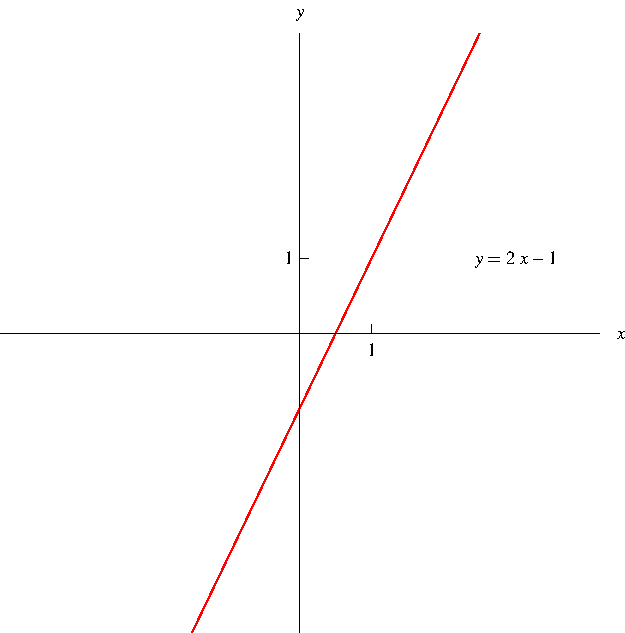
\includegraphics[height=6cm]{precalculus/pictures/01-02-line.pdf}%
Linear\phantom{Linear Qudratic Cubic Quartic Quintic}
}%
\only<handout:2| 2>{%
%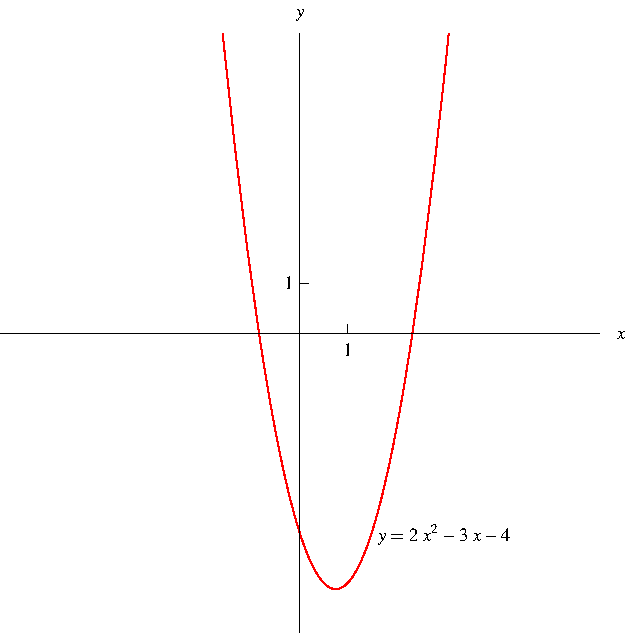
\includegraphics[height=6cm]{precalculus/pictures/01-02-parabola.pdf}%
Quadratic\phantom{Linear Qudratic Cubic Quartic Quintic}
}%
\only<handout:3| 3>{%
%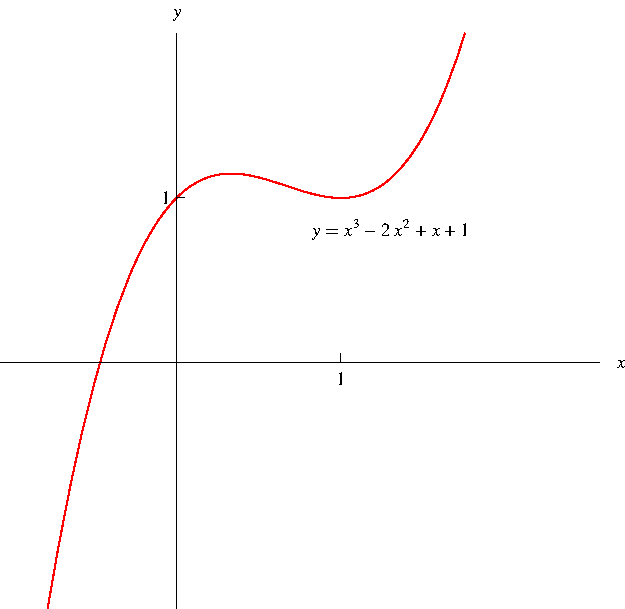
\includegraphics[height=6cm]{precalculus/pictures/01-02-polya.pdf}%
Cubic\phantom{Linear Qudratic Cubic Quartic Quintic}
}%
\only<handout:4| 4>{%
%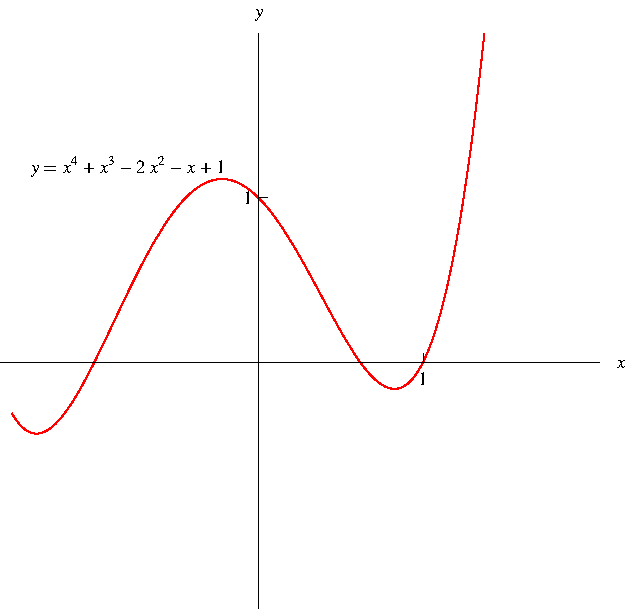
\includegraphics[height=6cm]{precalculus/pictures/01-02-polyb.pdf}%
Quartic\phantom{Linear Qudratic Cubic Quartic Quintic}
}%
\only<handout:5| 5>{%
%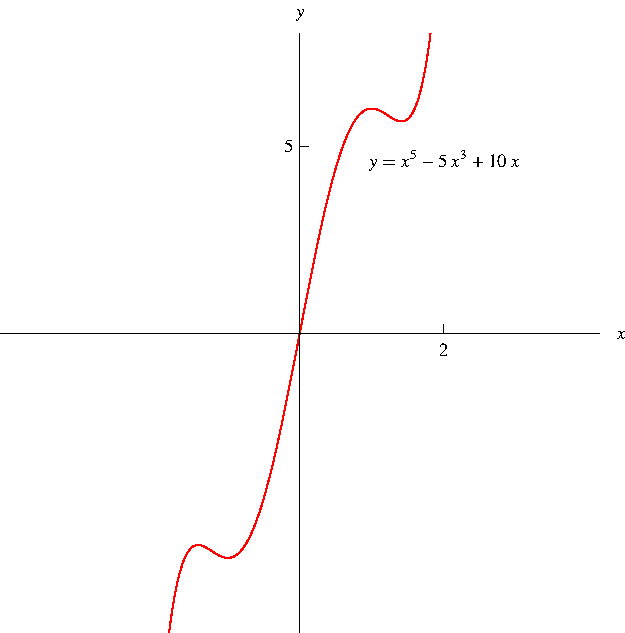
\includegraphics[height=6cm]{precalculus/pictures/01-02-polyc.pdf}%
Quintic\phantom{Linear Qudratic Cubic Quartic Quintic}
}
\end{frame}
% end module polynomials
